The aim of this chapter is to review how the system is tested in order to assess its quality as a whole. The three phases of the pipeline are analysed separately, with an emphasis on the online retrieval phase that produces the output of the system. The type of database videos and query videos used to test the system is clarified before diving into the evaluation of the results, starting with the online retrieval phase, followed by the offline feature extraction phase and ending with the database pre-processing phase. These phases are analysed with the help of software evaluation tools, along with figures and graphs utilised for visual representations of the results. Finally, an online experiment is conducted to establish ground truth matching and compared to the system's own result.

%%%%%%%%%%%%%%%%%%%%%%%%%%%%%%%%%%%%%%%%%%%%%%%%%%%%%%%%%%%%%%%%%%%%
%%%%%%%%%%%%%%%%%%%%%%%%%%%%%%%%%%%%%%%%%%%%%%%%%%%%%%%%%%%%%%%%%%%%
%%%%%%%%%%%%%%%%%%%%%%%%%%%%%%%%%%%%%%%%%%%%%%%%%%%%%%%%%%%%%%%%%%%%

\section{Testing Data}

\subsection{Database Videos}

The system is tested using a database of 50 different videos, ranging from 7 to 14 seconds, as per requirements F25-F26. The database of videos is populated from scratch using free stock footage from \textit{Pexels Video}\footnote{Pexels Video: \url{https://www.pexels.com/videos/}}. The videos used to build the database are chosen from a rich library of videos encapsulating many different colours (e.g. bright, dark, warm, cold, colourful, etc.) and movements (e.g. still, motion, shaky, blurry, timelapses, etc.) to ensure diversification in the dataset. The database of videos used to test the system can be found in the \textit{``footage''} directory in the provided code.\\

Employing existing databases of videos for CBVR tasks such as the TRECVID\footnote{Text REtrieval Conference Video Retrieval Evaluation} dataset \cite{2018trecvidawad}, which is the best dataset for CBVR-oriented tasks, would have been ideal to measure the project's performance and to compare it with existing solutions for this task. However, these datasets are not publicly available and hard to obtain. For example, most of the referenced proceedings in the Bibliography that present solutions to CBVR tasks were conducted for the TRECVID conferences, meaning that the datasets used to test the systems were provided to the participants for testing and evaluating results. However, the NIST\footnote{National Institute of Standards and Technology, organiser of the annual TRECVID conference} does not provide these databases for external research. Other databases of videos exist, but target other computer vision tasks such as facial recognition or image retrieval rather than CBVR. Therefore, the previously mentioned custom database of 50 copyright-free videos is used to test this system.

%%%%%%%%%%%%%%%%%%%%%%%%%%%%%%%%%%%%%%%%%%%%%%%%%%%%%%%%%%%%%%%%%%%%

\subsection{Query Videos}

Various query videos are recorded to test the online retrieval phase of the system. These queries are mobile recordings of one of the database videos. Different types of queries listed in Section \ref{sec:design-query-video-processing} are used to test the limits of the system, including down-scaled (recording at a distance from the screen) and skewed queries (recording at an angle) coupled with minor camera movement due to shaking hands. These conditions ensure the realism of the queries if the system were to be developed as a mobile application.\\

%%%%%%%%%%%%%%%%%%%%%%%%%%%%%%%%%%%%%%%%%%%%%%%%%%%%%%%%%%%%%%%%%%%%
%%%%%%%%%%%%%%%%%%%%%%%%%%%%%%%%%%%%%%%%%%%%%%%%%%%%%%%%%%%%%%%%%%%%
%%%%%%%%%%%%%%%%%%%%%%%%%%%%%%%%%%%%%%%%%%%%%%%%%%%%%%%%%%%%%%%%%%%%

\section{Online Retrieval Phase Results Evaluation}

The results are evaluated by counting the number of true positives and false positives for each video query used to test the system. A true positive corresponds to an outcome where the system matches the query to the correct database video, while a false positive is an outcome where the system matches the query incorrect to an incorrect database videos. The number of true positives and false positives occurrences are counted for each histogram model and distance metric used per query. As detailed in the previous chapter at the end of Section \ref{sec:implementation-distance-measurements}, these are used to plot the probabilities of the most likely database video to match the query in the form of a percentage \%. Additionally, other measurements are made such as the runtime of the system, its scalability, and the comparison of the final results under different conditions.

%%%%%%%%%%%%%%%%%%%%%%%%%%%%%%%%%%%%%%%%%%%%%%%%%%%%%%%%%%%%%%%%%%%%

\subsection{Video Matching Performance}

\subsubsection{Accuracy Measurements}

The system is first tested with down-scaled queries recorded at a straight angle to the screen. Shaky camera movement can be seen on the query videos, along with a considerable section of frame area not covering the actual video playing due to the distance to the screen. Despite these challenges, the queries still yield correct matches with high accuracy exceeding 50\% of true positives, with some excellent results that exceed 90\%. Figure \ref{fig:evaluation-downscaled-queries} depicts two examples of queries that incorporate the specified challenges, with the first query retrieving the correct video with 93.18\% accuracy, and the second one with 56.82\%. The important detail to notice in the left-hand side histograms is how the probability of the second closest match is much smaller than the probability of the closest match. Additionally, few alternative videos are marked as potential matches, with the first query only displaying two potential matches and the second query four potential matches. % recording1 and recording2

\begin{figure}[h] 
\centerline{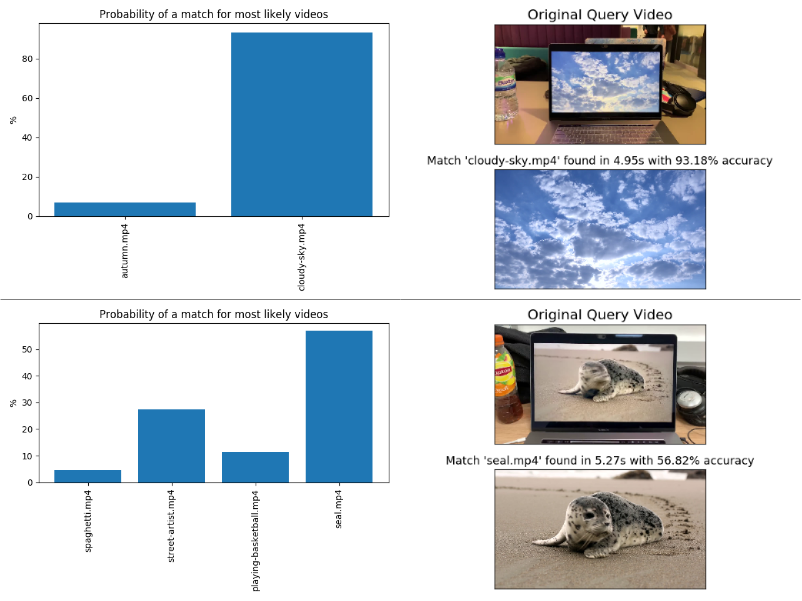
\includegraphics[width=\textwidth]{figures/evaluation/downscaled-queries.png}}
\caption{\label{fig:evaluation-downscaled-queries}Examples of results using down-scaled queries (recorded at a distance).}
\end{figure}

Next, skewed queries recorded at an angle from the screen playing the database video are tested. These tested queries also include all of the challenges mentioned in the first test, such as down-scaling (recording at a distance) and unstable footage. Despite the increased challenge presented by the skewed query, the accuracy of the matches still exceed 50\% and reach as high as 75\% despite poor quality queries. Figure \ref{fig:evaluation-skewed-queries} portrays examples of skewed queries. The first query filmed from the left side of the screen is identified as the correct match with 56.82\% accuracy, while the second query filmed from the right wide of the screen is identified as the correct match with 75\% accuracy. Observing at the left-hand side histograms in Figure \ref{fig:evaluation-skewed-queries}, it can be noticed that skewed queries cause the system to produce more potential video matches. Indeed, the first query produces six potential videos matches, which are quite different from the mainly-green \textit{``butterfly''} query, e.g. the main colours in the \textit{``autumn''} and \textit{``dunes''} are not green. This contrasts with the non-skewed queries that produce less potential matches. Nevertheless, the probability of the closest match remains greater than the probability of the second closest match despite the skewed query. % recording3 and recording8

\begin{figure}[h] 
\centerline{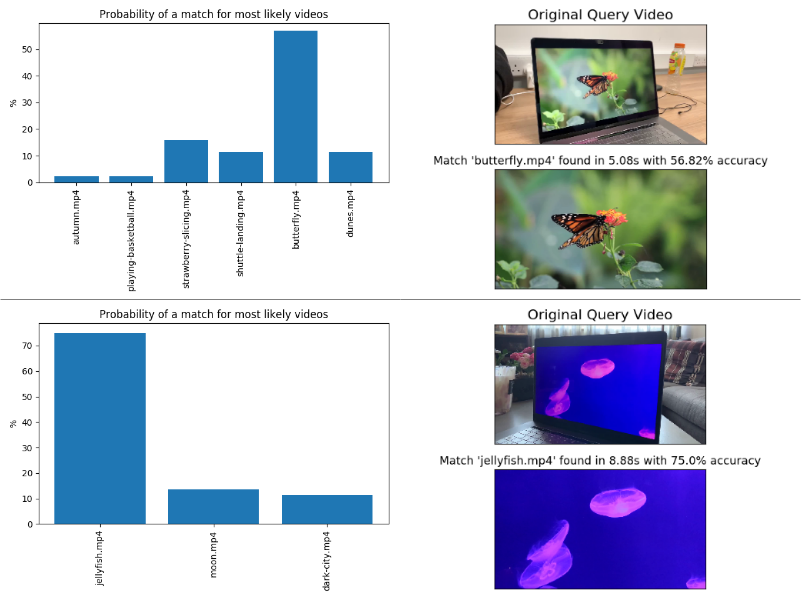
\includegraphics[width=\textwidth]{figures/evaluation/skewed-queries.png}}
\caption{\label{fig:evaluation-skewed-queries}Examples of results using skewed queries (recorded at an angle).}
\end{figure}

Although, the results demonstrated in the first two tests using down-scaled and skewed queries portrayed positive results with more than 50\% true positives, some queries result in a poorer accuracy, reaching a minimum of 45.5\% for a correct match, as shown in Figure \ref{fig:evaluation-poor-accuracy-query}. This low accuracy is partly caused by a combination of factors that are further explored in the next paragraph. % recording5

\begin{figure}[h] 
\centerline{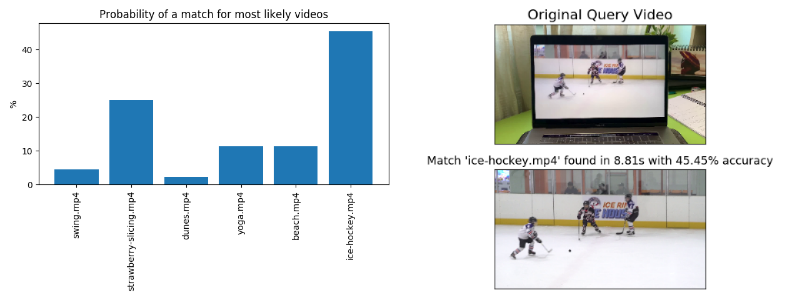
\includegraphics[width=\textwidth]{figures/evaluation/poor-accuracy-query.png}}
\caption{\label{fig:evaluation-poor-accuracy-query}Examples of results with poor accuracy.}
\end{figure}

%%%%%%%%%%%%%%%

\subsubsection{External Factors Observations}
\label{sec:evaluation-observations-online-phase}

External factors directly affecting the quality of the query can drastically influence the accuracy of the system, and even produce wrong matches. These factors are causes by the conditions of the environment rather than by the actual recording's quality.\\

The first noticeable environmental factor that causes the system to produce low-accuracy results and possibly wrong matches is the lighting in the room. While testing the system with different queries, the system had trouble coping with queries recorded at night-time in low luminosity environments. Indeed, during the filming of the queries at night-time, the lamps in the room produced warm white light with colour temperatures ranging between 2000K and 3000K\footnote{What is colour temperature? \url{http://www.westinghouselighting.com/color-temperature.aspx}}, which corresponds to orange/yellow light. These caused an alteration of the overall colour of the recorded screen, leading to the histograms to shift towards yellow/orange colours. This shift provoked the query's average histograms to be very disparate from the original database video's histograms, ultimately causing the system to generate the wrong input. Two cases of the consequences of this type of environment are illustrated in Figure \ref{fig:evaluation-yellow-light-queries}.\\ % recording4 and mismatch1

\begin{figure}[h] 
\centerline{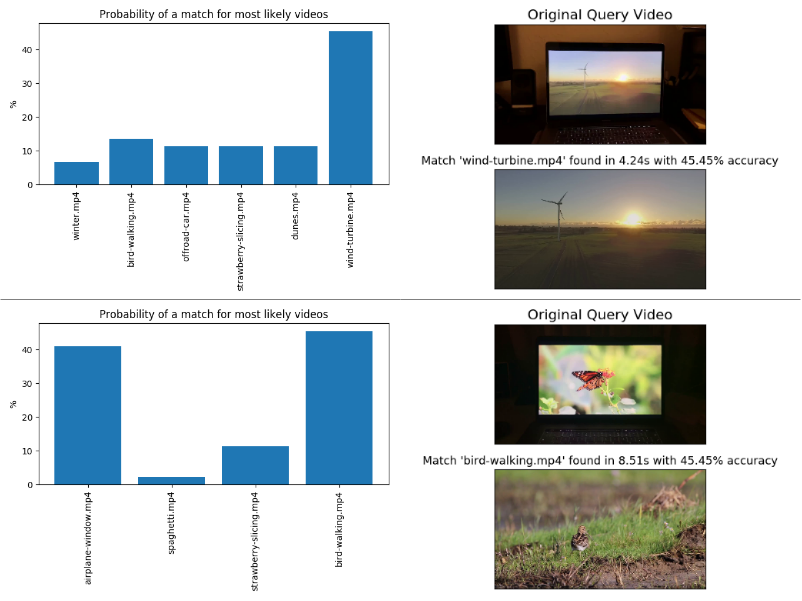
\includegraphics[width=\textwidth]{figures/evaluation/yellow-light-queries.png}}
\caption{\label{fig:evaluation-yellow-light-queries}Examples of results using queries recorded in a low-light environment.}
\end{figure}

The query from the first case (top of Figure \ref{fig:evaluation-yellow-light-queries}) is matched to the correct database video, but with a very low accuracy of 45.45\%. Furthermore, the system found five other potential matches, most with shades of yellow/orange colours (e.g. \textit{``dunes''}, \textit{``bird-walking''} and \textit{``offroad-car''}). The second query used from Figure \ref{fig:evaluation-yellow-light-queries} does not even find the correct match, pairing the \textit{``butterfly''} query to the \textit{``bird-walking''} video. The system does not even list the correct video as a potential match and moreover places the closest and second closest matches near each other (within 5\%). After watching the second query of the butterfly in more detail, it can be noticed that the dark environment is source to another factor. Due to the poorly lighted room, the luminosity of the screen stands out more, which can in turn shift the intensity of the pixels in the histogram towards the right (toward a value of 255). This contributes to the poor accuracy of the system in such conditions.\\

The second noticeable external factor is the presence of light reflections on the screen displaying the database videos. This factor, which is already probed in Section \ref{sec:design-query-video-processing} Figure \ref{fig:difference-query-video-issues}, depends on the positioning of the light source and the camera recording the query. Based on these, light glares might appear on the screen, greatly affecting the accuracy of the system as new colours appear on the screen, causing the histograms' pixel intensities to converge towards that new colour. Two cases reproducing the consequences of the light glares on the screen are represented in Figure \ref{fig:evaluation-light-reflection-queries}.\\ % recording7 and mismatch2

\begin{figure}[h] 
\centerline{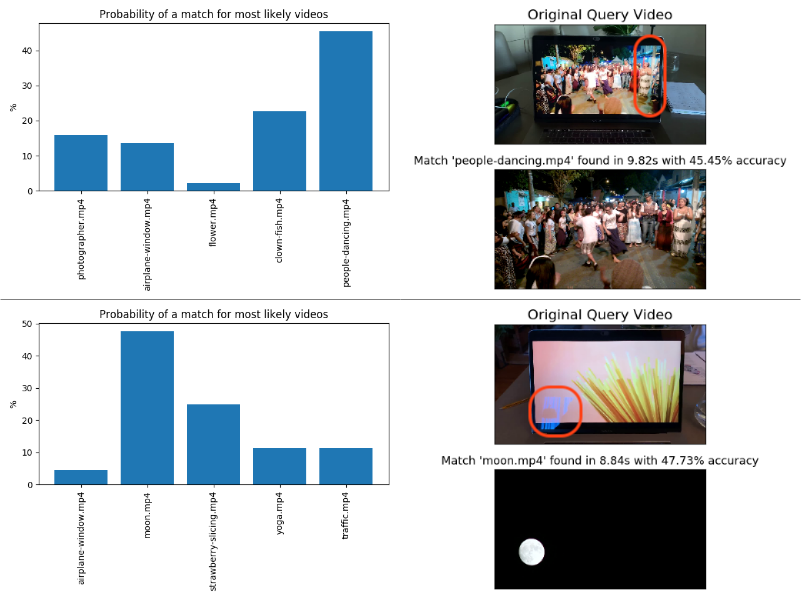
\includegraphics[width=\textwidth]{figures/evaluation/light-reflection-queries.png}}
\caption{\label{fig:evaluation-light-reflection-queries}Examples of results using queries recorded with light reflections on the screen.}
\end{figure}

The first query of \textit{``people-dancing''} is correctly matched to its database video regardless of the light glare on the right-hand side of the screen (highlighted in red), but again with a low accuracy of 45.45\%. The system detects potential matches in videos that are quite distant to the query video, such as \textit{``airplane-window''} or \textit{``flower''} which both have shades of blue similar to the glare. The second query of \textit{``spaghetti''} is matched to the wrong video, and is not even listed as a potential match despite its unique combination of yellow and pink colours because of the larger light glare in the bottom right of the screen (highlighted in red).\\

This section depicted the worst case performances of the system under difficult conditions, all caused by different lighting factors such as the colour of the light or the reflection of light on the screen playing the database videos. The next section critiques the combination of histogram models and distance metrics in more detail.

%%%%%%%%%%%%%%%%%%%%%%%%%%%%%%%%%%%%%%%%%%%%%%%%%%%%%%%%%%%%%%%%%%%%

\subsection{Histogram Models and Distance Metrics Analysis}

Reflecting on the results laid out in the previous section, a few analytical words can be shared regarding the combination of the histogram models and the distance metrics used to compute the results.\\

First, regarding the histogram models, the HSV histogram model was by far the most performant one, followed by the RGB histogram model in some cases and the least performant greyscale histogram model. 

Regarding the distance metrics used to calculate the difference between the query's histograms and the database videos' histograms, some performed better than others

\begin{comment}
analyse results of RGB, grey scale and HSV histograms with the 6 different histogram matching methods. which work best? in which scenarios? (use the 10 previous results to show this)

EMD and energy dist always find correct asnswer (explains the 45.45\% as lowest accurcy)

removing KL divergence metric greatly improved accuracy. (using less metric to use the ones for the job). KL divergence NEVER found correct match, not meant to be used a distance metric (show example of removing KL div and alternate chi square with past examples and new one)

improved cloudy-sky,
improved butterfly skewed

greyscale almost never finds a correct matc. Out of the 4 measurements, the maximum it finds is 2
\end{comment}

%%%%%%%%%%%%%%%%%%%%%%%%%%%%%%%%%%%%%%%%%%%%%%%%%%%%%%%%%%%%%%%%%%%%

\subsection{Runtime Measurements}

The runtime of each of the ten query videos used to test the system in the previous sections is plotted in a graph which can be found in Figure \ref{fig:evaluation-runtime_plot}. A few points can be made based on this graph. First, the runtime never exceeds 10s, thus fulfilling requirement F13. Second, the difference between the 1080p query videos and lower-quality 720p query videos' runtime is almost halved, with the runtime of 720p queries averaging 4.89 seconds and the runtime of 1080p queries averaging 8.91 seconds. However, the accuracy of system when processing the 720p queries is as high as the accuracy of the 1080p queries. Indeed, the \textit{``cloudy-sky''} query yields an accuracy of 93.18\%, while the accuracy of the \textit{``jellyfish''} query yield 75\% true positives. This crucial measurement reveals that using higher-quality does not necessarily translate to better results, meaning that any decent mobile device camera can be used with the system to generate descriptive histograms.

\begin{figure}[h] 
\centerline{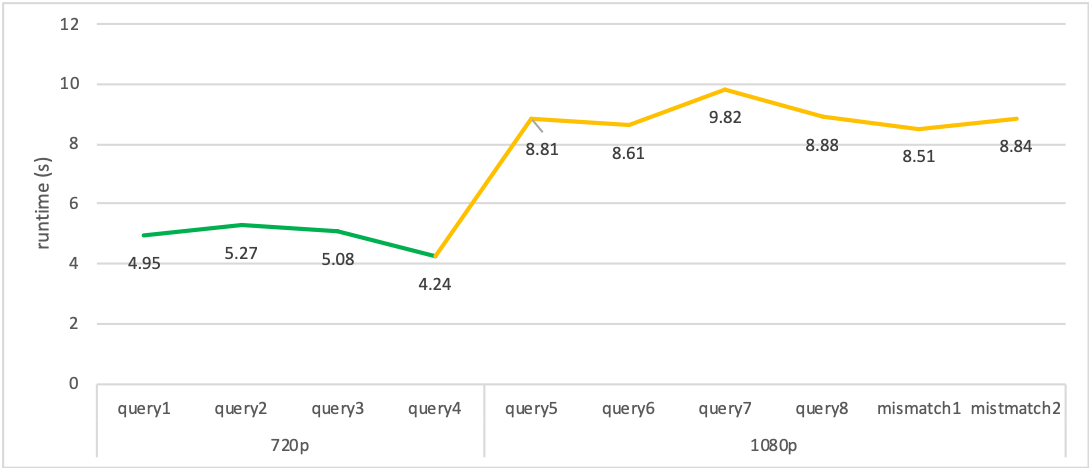
\includegraphics[width=\textwidth]{figures/evaluation/runtime_plot.png}}
\caption{\label{fig:evaluation-runtime_plot}Graph depicting the runtime for each query used to test the system, along with the resolution of each query.}
\end{figure}

%%%%%%%%%%%%%%%%%%%%%%%%%%%%%%%%%%%%%%%%%%%%%%%%%%%%%%%%%%%%%%%%%%%%
%%%%%%%%%%%%%%%%%%%%%%%%%%%%%%%%%%%%%%%%%%%%%%%%%%%%%%%%%%%%%%%%%%%%
%%%%%%%%%%%%%%%%%%%%%%%%%%%%%%%%%%%%%%%%%%%%%%%%%%%%%%%%%%%%%%%%%%%%

\section{Offline Feature Extraction Phase Scalability}

Evaluating the offline colour-based feature extraction phase is more tricky than evaluating the online retrieval phase as the output is always the same between different runs: three averaged histograms for each database video. This phase is nevertheless essential as it decides how large the database of videos can be. Therefore, a quantitative measure can be used to determine the scalability of this phase and how large the database can be.\\

The measure used to estimate the scalability of the system is the runtime of the phase. The mean runtime for generating the three averaged histograms for each video in a database of 50 videos is 163 seconds. With the way the features are extracted and the feature vectors are generate, the growth of the system is linear as it is equal to $163/50=3.26$ seconds per video. Adding a 51st video to the database will increase the runtime by 3.26 seconds. To predict how large the database of videos can be, the runtime in hours is plotted in a graph starting with 50 videos and growing up to one million videos based on the previous linear calculations. The results can be found in Figure \ref{fig:evaluation-offline_phase_runtime_trendline}.

\begin{figure}[h]
\centerline{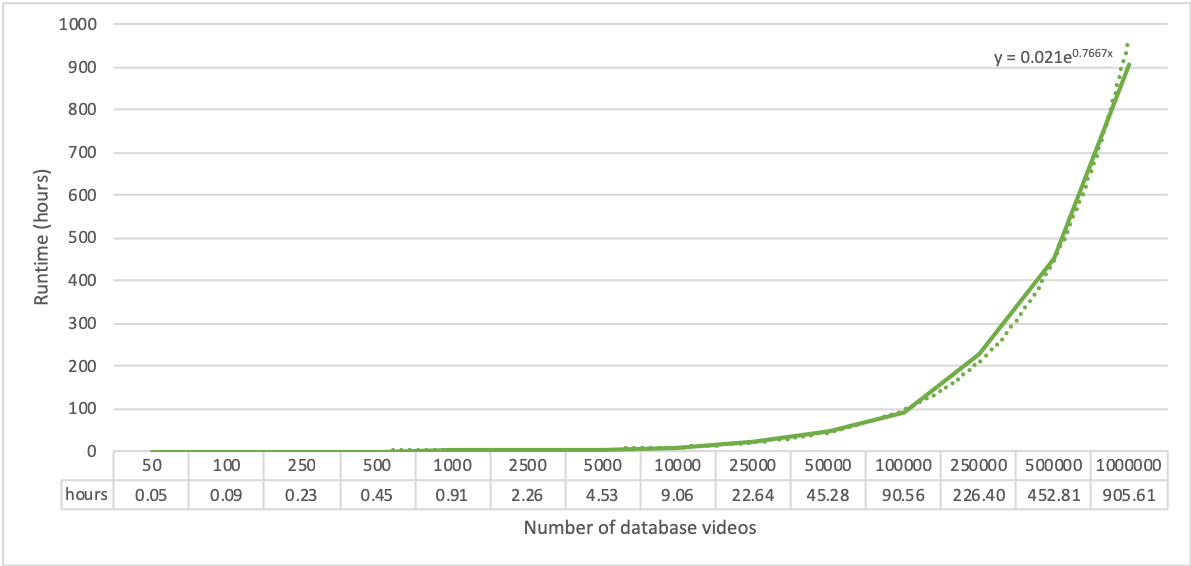
\includegraphics[width=\textwidth]{figures/evaluation/offline_phase_runtime_trendline.png}}
\caption{\label{fig:evaluation-offline_phase_runtime_trendline}Prediction of the offline colour-based feature extraction phase runtime for different database sizes. A trendline $y=0.021e^{0.7667x}$ can be fitted to the resulting series to determine the demand }
\end{figure}

These results clearly betray the demand of processing large databases of videos. Up until 1000 videos, the runtime of processing the database would be inferior to one hour. The runtime reaches 9 hours for reaching 10000 videos, which is still acceptable to calculate in a single execution. However, the runtime to process larger databases would need to be calculated in days rather than hours when the database reaches one million videos, with runtimes of $905.61/24=37.73$ days. This would be feasible with dedicated hardware running this phases through multiple batches and building the compact signature for each database video over time, but not for the current system.

%%%%%%%%%%%%%%%%%%%%%%%%%%%%%%%%%%%%%%%%%%%%%%%%%%%%%%%%%%%%%%%%%%%%
%%%%%%%%%%%%%%%%%%%%%%%%%%%%%%%%%%%%%%%%%%%%%%%%%%%%%%%%%%%%%%%%%%%%
%%%%%%%%%%%%%%%%%%%%%%%%%%%%%%%%%%%%%%%%%%%%%%%%%%%%%%%%%%%%%%%%%%%%

\section{Database Pre-Processing Test: Movie Segmentation}
\label{sec:evaluation-movie-segmentation-test}

The initial motivation behind the project being to create a CBVR system for feature-length movies, the phase dedicated to pre-process the database of movies is tested with a feature-length movie to observe how it can be segmented using the implemented shot boundary detection. The movie used for the test is Inception\footnote{Inception IMDb page: \url{https://www.imdb.com/title/tt1375666/}}, a 2h28 movie composed of 213098 frames in total. The shot boundary detection algorithm is tested once with the KL Divergence and once with the Intersection metric, as depicted in Figure \ref{fig:evaluation-inception_shot_boundary_detection_test}.\\

\begin{figure}[h] 
\centerline{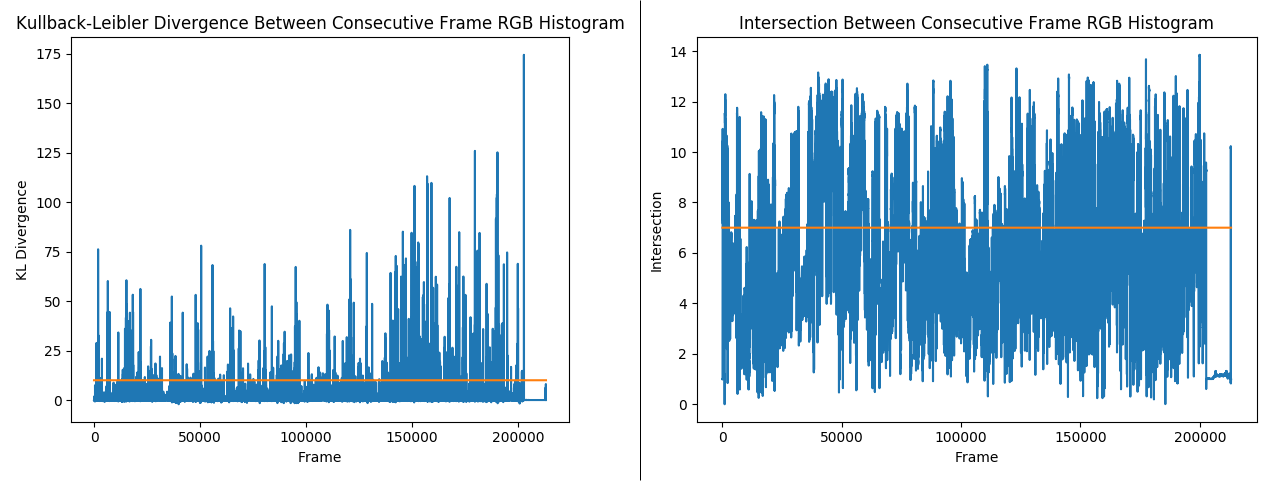
\includegraphics[width=1.15\textwidth]{figures/evaluation/inception_shot_boundary_detection_test.png}}
\caption{\label{fig:evaluation-inception_shot_boundary_detection_test}Result of the shot boundary detection algorithm on the Inception movie using the KL Divergence (left) and Intersection metric (right) between consecutive frames' RGB histograms.}
\end{figure}

The first test uses the KL Divergence to detect the difference between consecutive frames while employing a global threshold $t=10$, which detects a total of 661 different shot boundaries throughout the entire film in 2h29. Alternatively, the second test uses the Intersection metric while employing a global threshold $t=7$, which detects a total of 1730 shot boundaries 2h41. Although the difference between the two results seems considerable as the Intersection metric detects almost three times more shot boundaries than the KL Divergence, the difference between the two is actually quite small when considering the bigger picture. Indeed, the 661 shot boundaries represent only 0.31\% of the movie, while the 1730 shot boundaries represent 0.81\% of the movie. When considering that the goal of the database pre-processing is to segment the database videos in order to have less frames to process in the offline feature extraction phase, then cutting down the number of frames to process to less than 1\% is a satisfactory result that will greatly improve the results when working with long videos.\\

% In terms of runtime, the KL Divergence shot boundary detection took 2h29 to complete, while the intersection shot boundary detection test took 2h41 to complete. With the movie lasting 2h28, it takes slightly longer than the movie itself to process it for shot boundary detection. Therefore, treating a large database  

%%%%%%%%%%%%%%%%%%%%%%%%%%%%%%%%%%%%%%%%%%%%%%%%%%%%%%%%%%%%%%%%%%%%
%%%%%%%%%%%%%%%%%%%%%%%%%%%%%%%%%%%%%%%%%%%%%%%%%%%%%%%%%%%%%%%%%%%%
%%%%%%%%%%%%%%%%%%%%%%%%%%%%%%%%%%%%%%%%%%%%%%%%%%%%%%%%%%%%%%%%%%%%

\section{Comparison With Ground Truth Experiment}

An experiment with 20 participants was conducted to establish ground truth video matching. The experiment was conducted online through the use of Google Forms\footnote{Google Forms: \url{https://www.google.com/forms/about/}}. During the experiment, the users were first presented six different database videos to simulate the offline colour-based feature extraction phase. Next, they were shown one query video and asked to rank the six videos they watched from most likely to least likely to match the query video in order to simulate the online retrieval phase. The same six database videos and query video were then used with the system to compare with the participants' rankings. To render the matching task compelling, the six videos, which can be found in Figure \ref{fig:evaluation-online_experiment_dbvideos}, all have different shades of blue.

\begin{figure}[h] 
\centerline{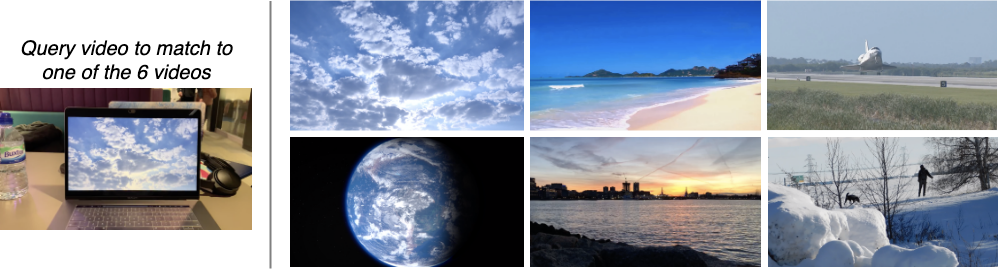
\includegraphics[width=\textwidth]{figures/evaluation/online_experiment_dbvideos.png}}
\caption{\label{fig:evaluation-online_experiment_dbvideos}The query video and the six database videos shown to the participants.}
\end{figure}

The results of the online experiment along with the results of the system are plotted in Figure \ref{fig:evaluation-ground_truth_vs_system_results}. The most essential aspect between the experiment's results and the systems results is that both ranked the correct video (\textit{``cloudy-sky''}) as the most likely video to match the query with 100\% accuracy, meaning that every participant matched the query to the correct database video, and so did the system for each histogram model and distance metric calculation. This confirms with certainty that \textit{``cloudy-sky''} is the correct match to the query. However, while observing the five other matches, it can be seen that they are not ranked in the same order between the ground truth and the algorithm. On the one hand, the results of the ground truth experiment ranks the other videos as 2: \textit{earth} 3: \textit{shuttle}, 4: \textit{winter}, 5: \textit{sunset} and 6: \textit{beach}. On the other hand, the results of the system ranks the other videos as 2: \textit{winter}, 3: \textit{earth}, 4: \textit{shuttle}, 5: \textit{beach}, 6: \textit{dusk}. Interestingly, despite the different rankings between the other videos, a parallel can be drawn between the accuracy for each match. Indeed, the participants and the system ranked the second closest match with 50\% accuracy, while they ranked the third closest match with the lowest accuracy (25\% for the participants and 22.7\% for the system). The common points between the ranking accuracies are through-provoking as they indicate similar behaviour between the participants and the system. As a matter of fact, the participants were asked what visual aspect of the video they considered the most when ranking the videos, and 80\% of them stated that they considered the colours of the query video to match it to the six other videos. This explains the similar accuracies between the matches, but the discrepancy in the ranking order could be explained by the fact that 70\% of the participants considered visual aspects other than colour when ranking the videos, such as motion, shapes, objects, sound and even semantic meaning.

\begin{figure}[h] 
\centerline{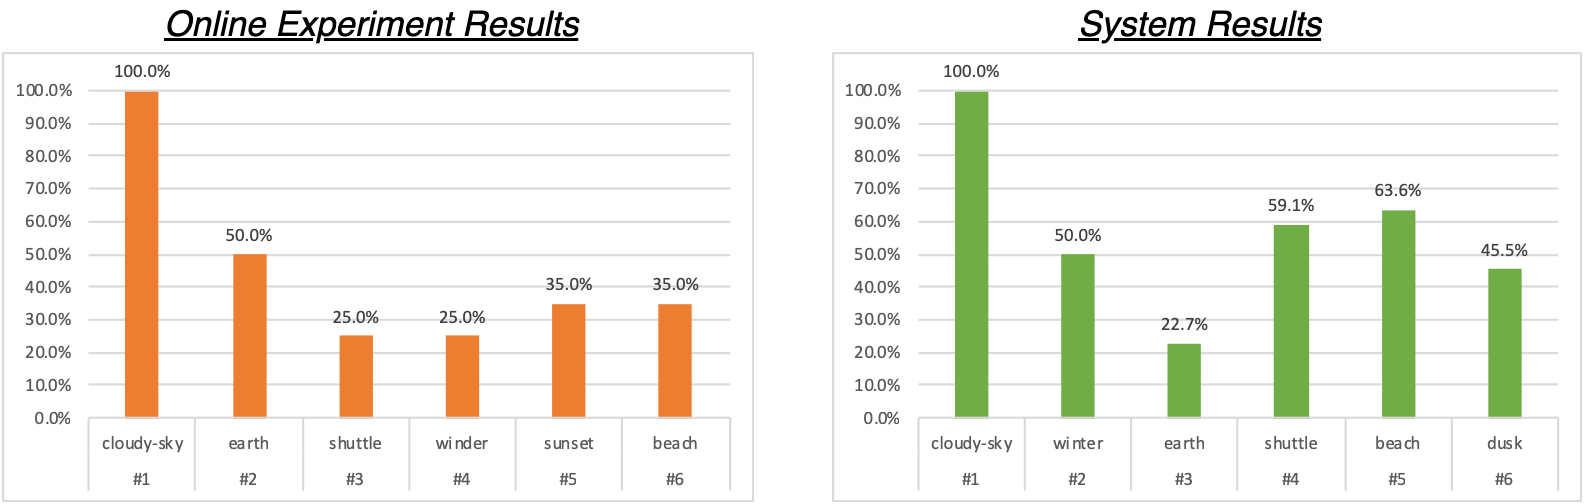
\includegraphics[width=\textwidth]{figures/evaluation/ground_truth_vs_system_results.png}}
\caption{\label{fig:evaluation-ground_truth_vs_system_results}Comparison of the online experiment results and the system's results.}
\end{figure}

Supporting documents covering the online experiment can be found in the appendix, including the Ethics Checklist in Appendix \ref{ch:appendix-ethics-checklist}, the Experiment Survey in Appendix \ref{ch:appendix-experiment-survey} and the experiments results in Appendix \ref{ch:appendix-survey-results}.

%%%%%%%%%%%%%%%%%%%%%%%%%%%%%%%%%%%%%%%%%%%%%%%%%%%%%%%%%%%%%%%%%%%%
%%%%%%%%%%%%%%%%%%%%%%%%%%%%%%%%%%%%%%%%%%%%%%%%%%%%%%%%%%%%%%%%%%%%
%%%%%%%%%%%%%%%%%%%%%%%%%%%%%%%%%%%%%%%%%%%%%%%%%%%%%%%%%%%%%%%%%%%%

\section{Summary}

todo